\documentclass[preprint]{aastex} 

\usepackage[top=1in, bottom=1in, left=1in, right=1in]{geometry}
\usepackage{amsmath}
\usepackage{graphicx}
\usepackage{mdwlist}
\usepackage{natbib}
\usepackage{natbibspacing}
\setlength{\bibspacing}{0pt}
\setlength{\parskip}{0pt}
\setlength{\parsep}{0pt}
\setlength{\headsep}{0pt}  
\setlength{\topskip}{0pt}
\setlength{\topmargin}{0pt}
\setlength{\topsep}{0pt}
\setlength{\partopsep}{0pt}
\setlength{\footnotesep}{8pt}
\pagestyle{empty}
\citestyle{aa}

\newcommand{\simgt}{\stackrel{>}{_{\sim}}}
\def\kperp{k_{\bot}}
\def\kpar{k_{\|}}
\def\k{{\bf k}}
\def\sky{{\theta}}
\def\HI{{H{\small I }}}
\def\HII{{H{\small II }}}
\def\xHI{{x_{\rm\HI}}}

%\usepackage{subfig}
%\usepackage[countmax]{subfloat}

\begin{document}
\title{Project Management Plan}

%A Project Management Plan should be submitted as a supplementary document, and may be up to 
%15 pages in length, although many programs will not need this much space. (Note that the solicitation 
%stated that the management plan should be provided in the Project Description; here we move it to its 
%own supplementary document so that it may be explicitly evaluated by reviewers.)  This section must 
%present a clear and thorough discussion of the project management structure and techniques that will 
%be applied. It may include, for example, a construction plan and schedule, a collaboration management 
%plan, a plan for managing telescope access, or any other pertinent management information. The 
%management plan should identify risks and describe their planned mitigation. If your proposed project 
%would have contributions from sources other than NSF, this section should clearly state both the total 
%cost, and the amount being requested from NSF.  

\section{Collaboration and Governance}
HERA builds upon the organization, tools and collaborations developed within the now merged 
PAPER and MWA-US groups.
In addition to the proposing collaborators in the {\em List of Partner Institutions},
HERA includes key partners in South Africa and the UK and is finalizing a collaboration with ASIAA.
\begin{table}[h]
\begin{tabular}{| p{.35\textwidth} | p{.6\textwidth} |}\hline
\textbf{Institution (location)} & \textbf{Role} \\ \hline
SKA-SA (Cape Town, SA) & Partner in site development, logistics, support, science \\ \hline
University KwaZulu Natal (Durban, SA) & Partner in science and support \\ \hline
Cavendish Laboratory (Cambridge, UK) & Partner in development etc \\ \hline
Academia Sinica Institute for Astronomy and Astrophysics (Taipei, Taiwan) & Science, development \\ \hline
\end{tabular}
\label{tab:otherpartners}
\end{table}

\begin{figure}[h]
\centering
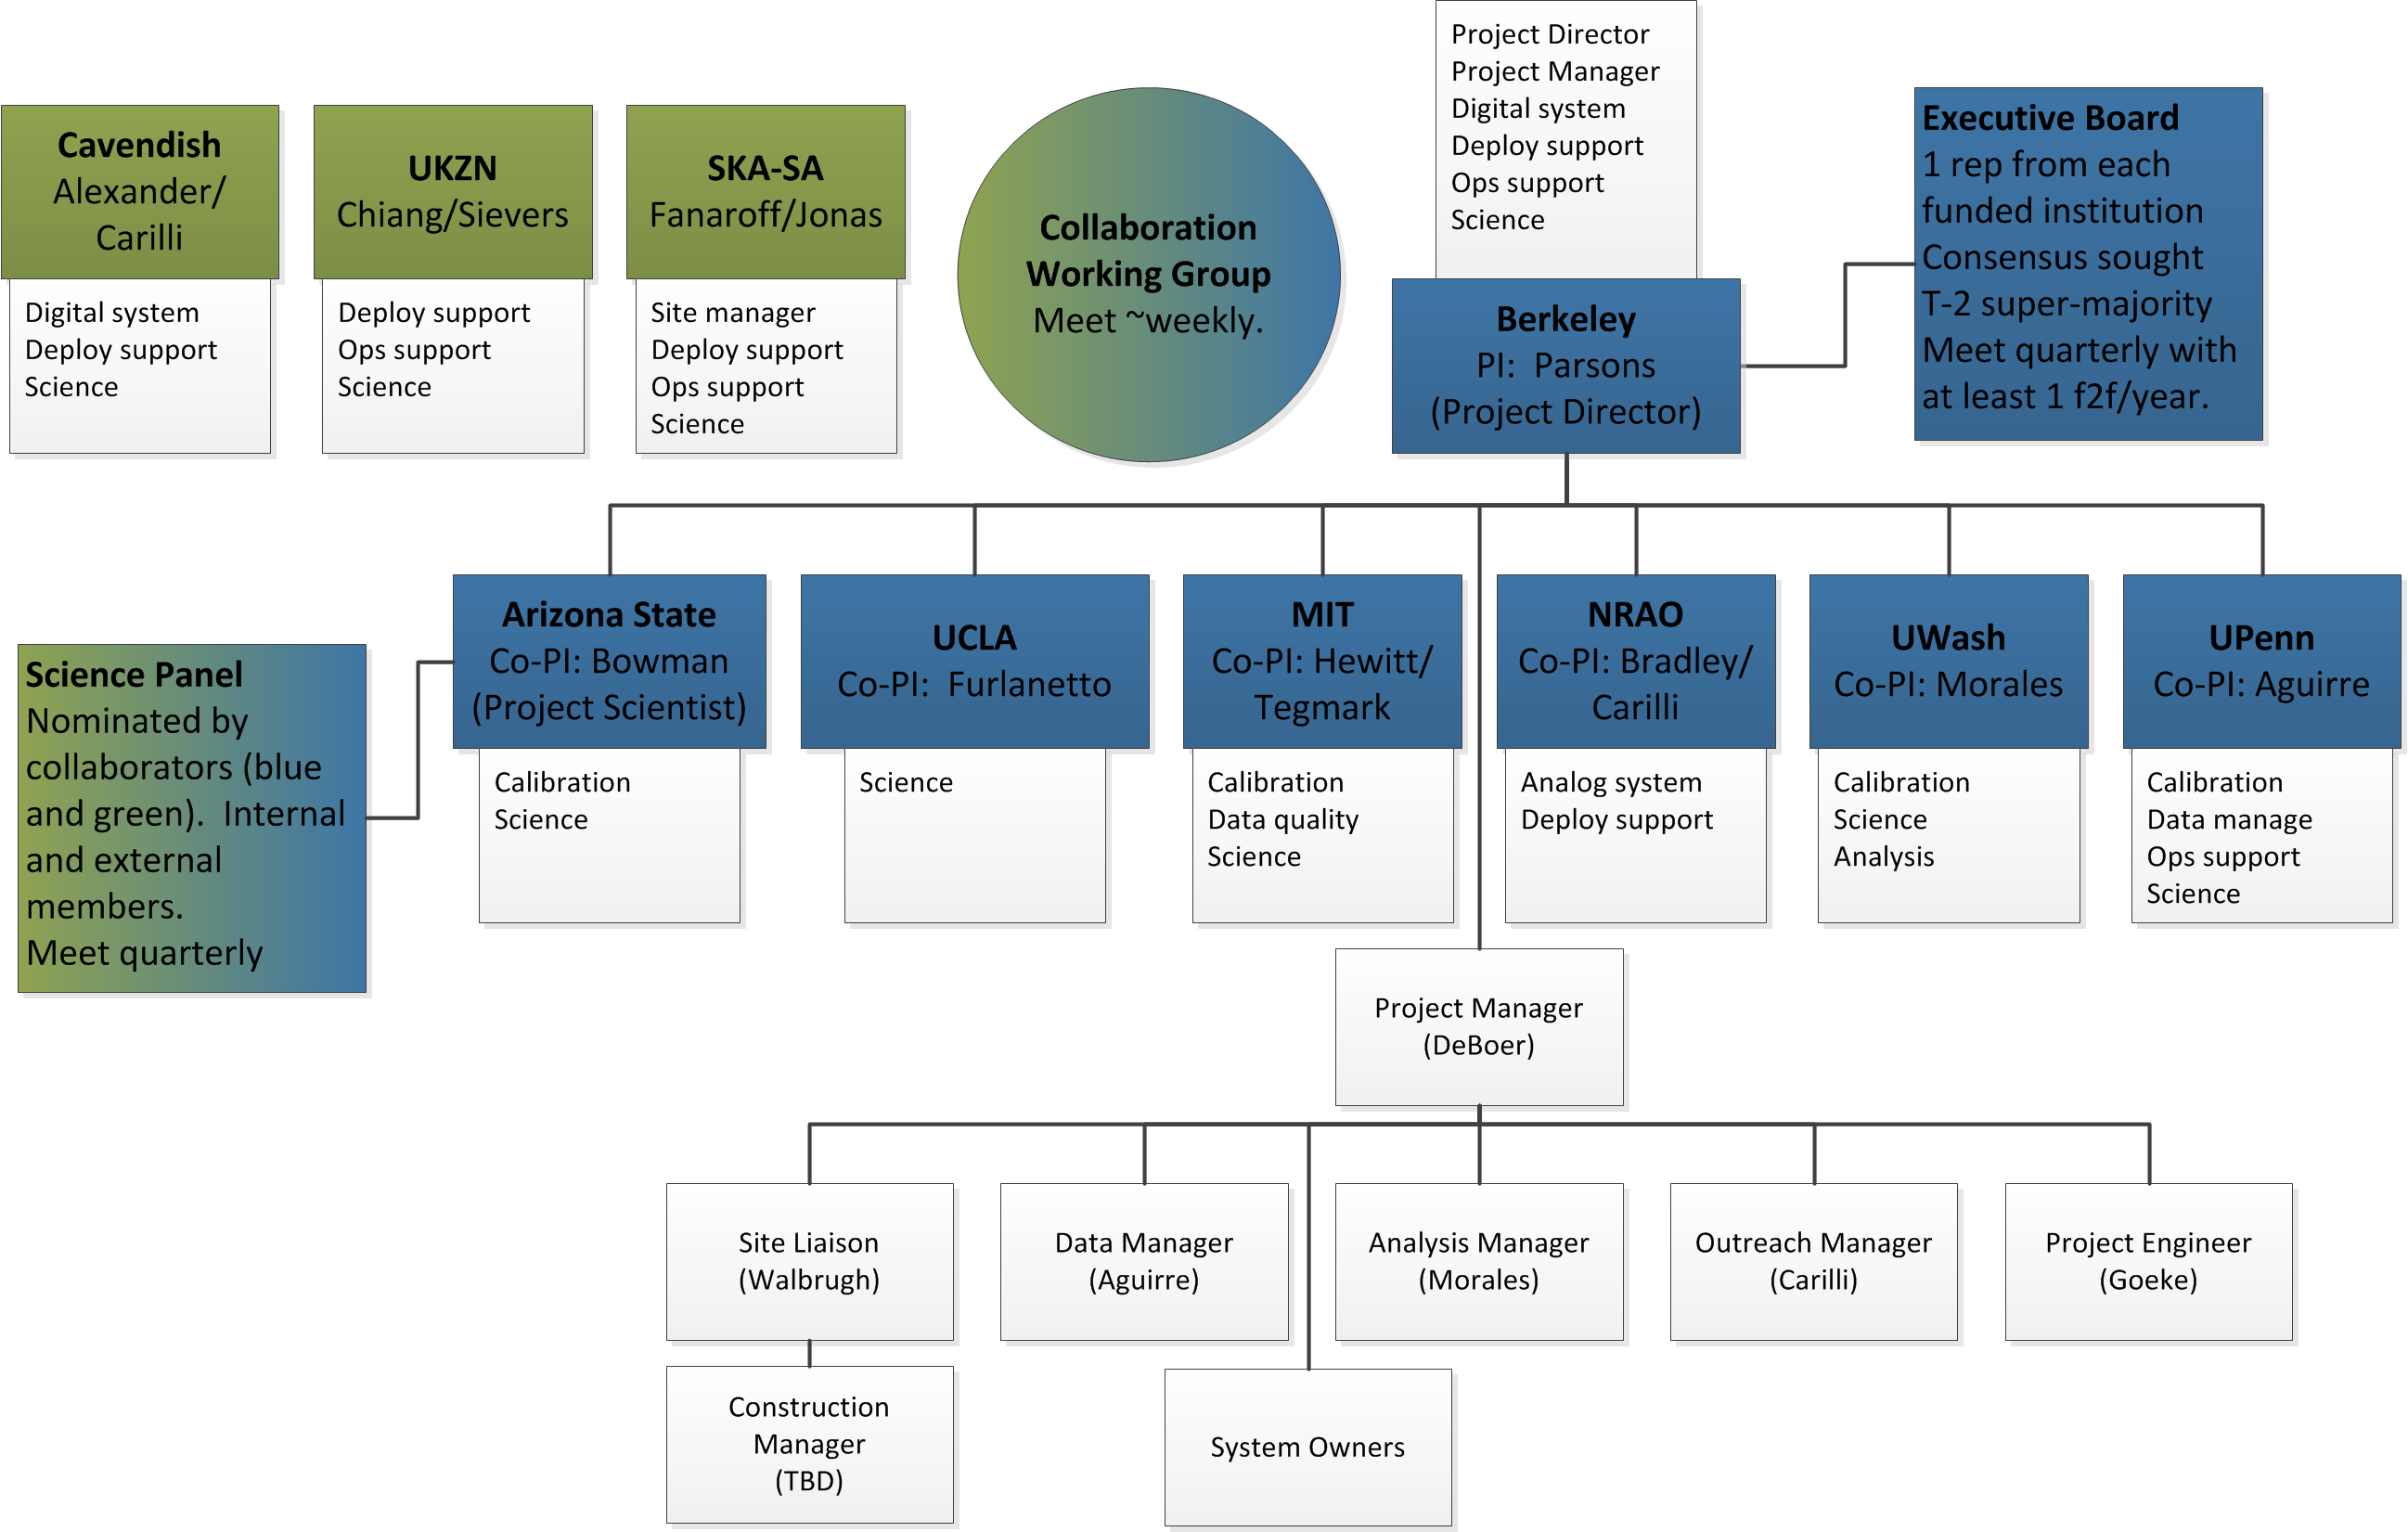
\includegraphics[width=\textwidth]{plots/org.png}
\label{fig:org}
\caption{Org chart showing the collaboration, governance and management.}
\end{figure}

Figure \ref{fig:org} shows the governance and management of the proposed work. 
The Executive Board serves as the governing board and has authority over the science 
Requirements\footnote{{\em Requirements} are the science and operational level requirements as
specified and managed by the Board.  {\em Specifications} are the system requirements
specified by the System Owners.}, the Scope of the science goals and Milestones. It consists 
of one voting representative from each of the funded partners, which typically will be the 
senior scientific partner at the institution. The Board is chaired by the Project Director. Though 
generally operating on concensus, if matters come to a vote a ``T-2''\footnote{T-2 means that 2
or more must vote against to defeat a motion.} supermajority will be required. The
Executive Board will meet at least quarterly, with at least one face-to-face meeting
per year. The Board is responsible for producing the NSF annual report.

A Science Panel, chaired by the Project Scientist or designate, will meet at least
quarterly to provide advice on the science (scope, progress, support, ). The
composition is determined by the Executive Board, and membership is open to anybody
the Board deems advisable and is willing to serve. Under the auspices of the Science
Panel, one face-to-face workshop will be held per year, rotating its location among
the partners.

The Collaboration Working Group comprises individuals named by the partner
institutions and will meet approximately weekly to review the project. It is chaired
by the Project Director or designate and will discuss any and all relevant aspects of
the project. It represents the primary method of frequent communication between the
partners.

\subsection{Communication}
Meetings (telecon Blue Jeans/Webex)  workshop, common repositories, web-site, wiki, email

Berkeley provides full access to the Blue Jeans network-conferencing system for hosting meetings, including
video, simple and effective desktop sharing, and multiple access methods.  Other partners have access to Webex,
which is also used.  These tools are routinely and effectively used by the partners already.

US-SA

Conference side meetings etc

\subsection{Publication}


\section{Management}
Figure \ref{fig:org} also shows the management structure.   A Project Manager has
overall responsibility for planning and tracking to achieve the agreed upon
milestones and budget. The Project Manager will brief the Executive Board at each
meeting to summarize the state of the project.  David DeBoer from Berkeley will serve
as the Project Manager.

The Site Manager/Liaison

The Data Manager has responsibility for ensuring data quality as archived at the KAPB and 
Penn.  James Aguirre from Penn will serve as the Data Manager.

The Analysis Manager has responsibility for ensuring that the analysis pipelines are super terrific.
Miguel Morales from Washington will serve as the Analysis Manager.

The Project Engineer has responsibilty for ensuring that Components and Systems meet their overall
Specifications and that Interfaces are properly addressed.  Bob Goeke from MIT will serve as the
Project Engineer.

\subsection{Project Structure}
The project comprises {\em Components}, which are the physical deliverables, and {\em Systems},
which are logical groupings to achieve a function. Systems may be hardware, software
or both. Systems need not be disjoint collections of Components. Each System has an
{\em Owner}, who is responsible for the System meeting its specifications and satisfying
its interface requirements.

Components will likely span multiple Systems. The Project
Manager serves as the Owner of the South Africa-based hardware Components, the data
manager is the Owner of the US-based hardware Components and the analysis manager is 
the Owner of the analysis software.  The Component Owners work with the System Owners 
to meet the Components functional specifications.  In practice there is a great deal of overlap
between the Components and Systems, making this arrangement practical but it also allows
a mechanism to ensure more ``eyes'' on the overall system.

\subsection{Management Tools}
The architecture, requirements/specifications, interfaces, budget, milestones, work breakdown structure
(WBS) and system documenation are in a common shared repository, along with collaboration
documentation.  This shared repository is referred to as the \textbf{Project Book}.  Architecture, requirements/ 
specifications, interface and milestone information reside in a \LaTeX-based database with full traceability
and python scripts for flow-down throughout the documentation.  Budget and WBS are in Microsoft
Excel and Microsoft Project with python script readers for flow-down throughout the documentation.

An executive script ensures that all scripts are executed and up-to-date formatted \LaTeX pdf documentation
files are produced.  These include auto-generated architecture, requirement/ specification, 
interface control, and milestone documentation, budget and WBS summary documents, as well as
flow-down files into the architecture for traceability. 
In addition to the auto-generated reports, System and  Component Owners write the narrative 
documentation referencing the database items as variables ({\em e.g.} requirements, interfaces, etc).
Additional scripts may be written as needed to access the system for customized reports.

Frequent telecons with modern conferencing systems are absolutely essential collaboration tools, 
as discussed above, and liberal use of these systems will continued to be applied.

The Project Book remains the definitive record, but use of a wiki for posting material and hosting
discussions etc is an important component.  The project has full access to wiki tools, and has been
using collaborative wikis in the ongoing collaboration.

Additional common repositories host the software developed by the project.  This allows access to all members,
as well as full revision control.

Schematics:  visio, technical

python, git/github

Financial BFS

\subsection{Change Control}
Change requests are initiated by an e-mail to the Project Manager indicating the proposed change
and reasons why it is necessary.  Changes may be of the Architecture, Scope, Requirements/ Specifications
Milestones and/or Interface as documented in the Project Book.  The Project Manager will investigate the 
impact of the proposed change and make a recommendation which may be provided to different bodies, 
depending on the scope of the change.  The Project Manager may initiate a change request by appropriately 
formulating and sending on a recommendation.

As mentioned above, the Executive Board controls Requirements, Scope and Milestone change requests
and they receive recommendations regarding these items.  If accepted, the Board will instruct the Project Manager to 
propagate the change within the management system and communicate this change to the partners.

Other change request recommendations will be provided to the impacted Owners of Systems and
Components and accepted on a consensus basis of the impacted Owners and Project Manager.  
In the event that consensus is not reached, the Project Director remains the final arbiter.  The Project 
Director may overrule consensus by approval of the Executive Board.  If accepted, the Project Manager 
will institute the change and communicate appropriately throughout the project.

\section{Construction}
plan, schedule, contract summary, milestone summary

\section{Analysis Management}

\section{Budget Overview}

\section{WBS Overview}

\section{Risk}

\end{document}
